% Tämä tässä on LaTeX-lähdekoodia. Prosenttimerkki aloittaa kommentin, jonka
% jälkeinen osa rivistä ei näy julkaistavassa dokumentissa.

% Kommentteja voi laittaa tarpeen mukaan - aivan kuin ohjelmakoodiin. Kaikki,
% mikä ei ole kommenttia, on LaTeX-järjestelmän tulkittavaksi tarkoitettua
% merkintää rakenteiselle dokumentille.

% LaTeX on kummallinen, mutta valtavan käyttökelpoinen vekotin, missä voit
% kirjoittaa ja siinä seassa tarpeen mukaan vähän ohjelmoida tuottaaksesi
% ladotusta tekstistä ja asemoiduista kuvista koostuvan julkaisun - ensialkuun
% nyt vaikkapa gradun. Kaikki on kovin automaattista ja näppärää varsinkin
% sitten, kun tekstin, lähdeviitteiden ja dokumentin sisäisten ristiviittausten
% määrä alkaa lähennellä mielekkään tieteellisen tutkimuksen tarpeita.

% Tämä pohja on muokattu gradu3 -dokumenttiluokan esimerkkigradusta ITKY4000:n
% tarpeisiin syksyllä 2019. Tästä on poistettu kaikki ylimääräinen, ja tähän on
% jätetty vain minimaalinen pohja ITKY4000:n oppimispäiväkirjan 4. osan
% toteuttamista varten.

% Tarkoitus on tarjota kaikille syksyn 2019 itkyttelijöille pehmeä ensikosketus
% LaTeXiin, jolla meidän omat kandimme ovatkin jo tehneet yhden tutkielman
% aiemmin.

% Ensikosketuksessa voit etsiä tästä tiedostosta kohdat, jotka pitää muuttaa,
% että mallina annetusta oppimispäiväkirjasta tulee esimerkin sijaan omasi. Sama
% prosessi tehdään yleensä teknisten ja matemaattisten alojen
% tutkimusartikkeleille: Ladataan lehden julkaisijan nettisivulta mallipohja ja
% aletaan muokata sitä kommenttien ohjaamana. Tulee just sen muotoinen artikkeli
% kuin kyseiseen lehteen halutaan. Ja tästä nyt tulee just sen muotoinen kuin
% ITKY4000:ssa halutaan :).

% Kun aikanaan aloitat oikean gradun tekemisen, hae netistä sen hetken uusin
% versio dokumenttiluokasta, laita pohjadokumenttisi mahdollisimman nopeasti
% versionhallintaan ja tee sille myös etävarasto (esimerkiksi privaatti repo
% githubiin, gitlabiin tmv.) ettei laitevika tai muu ulkoinen syy pääse
% tuhoamaan gradua varten tekemääsi työtä eivätkä versiot mene sekaisin. (Siinä
% vaiheessa koulutusta toivottavasti ymmärrät, mitä äskeinen sanahelinä
% tarkoittaa, ja osaat tehdä sen heittämällä sinä kauniina iltana, kun gradun
% aloitus tuntuu erityisen ajankohtaiselta:))

\documentclass[utf8]{gradu3}
% For any *foreign* student in there.. You may write in English, in which case
% you should use the following line instead:
% \documentclass[utf8,english]{gradu3}

% Suomalaiset kirjoittavat suomeksi! (==Finns write in Finnish!)

\usepackage{graphicx} % kuvien mukaan ottamista varten; tarvitaan.

%\usepackage{amsmath} % hyödyllinen jos tekstisi sisältää matikkaa, % ei
%                     pakollinen

% ... ja niin edelleen, oikeassa gradussa... tässä otetaan mukaan tarvittavia
% lisäosia erilaisten juttujen latomiseen dokumenttiin.

% HUOM! Tämän tulee olla viimeinen \usepackage koko dokumentissa!
\usepackage[bookmarksopen,bookmarksnumbered,linktocpage]{hyperref}

\addbibresource{opk4.bib} % Lähdetietokannan tiedostonimi; tarvitaan.

% ^
% |
% +---- yllä olevat ovat teknisiä määritelmiä, joilla voi säätää kaikenlaista.

% LaTeX-dokumentin varsinainen sisältö alkaa aina \begin{document} ja päättyy
% \end{document}.

% Pro-tip: mallipohjan voi jättää LaTeX-lähdekoodin loppuun malliksi erilaisten
% juttujen tekemisestä teknisesti. Sieltä voi ammentaa copy-paste-modifyllä niin
% ei tarvitse niin paljon tehdä KVG-menettelyä LaTeX-temppujen tekemiseksi.
% Miten? Laittamalla vaan \end{document} jo siihen kohtaan, missä oma
% tämänhetkinen tuotos loppuu. LaTeX-järjestelmä lopettaa lukemisen käskystä
% siihen.

\begin{document}

% Seuraavaksi tulevat nimiötiedot täytyy aina laittaa. LaTeX-pohjat helpottavat
% muistamaan, mitkä nimiötiedot julkaisuun, esimerkiksi graduun, tarvitaan
% julkaisijan asettamien sääntöjen mukaan. Yleensä aloitetaan kirjoittaminen
% vaihtamalla nimiötiedot omiksi, ja ryhdytään sitten raapustelemaan sisältöä
% mallitekstinä olevan diibadaaban ja/tai muoto-ohjeistuksen tilalle.

\title{Miten kissa lähti liikkeelle, noin niinku omasta mielestä}
\translatedtitle{What hit the fan -- in my own words (usually a more precise translation of the Finnish title)}

\author{Paavo Nieminen} %  <-- oma nimesi tietysti tähän, ja yhteystiedot:
\contactinformation{\texttt{paavo.j.nieminen@jyu.fi}} \studyline{Ohjelmisto- ja
tietoliikennetekniikka} % <-- voi vaihtaa oman tuohon.

% --------------------------------------------------------------------
% Tiivistelmä ja avainsanat voivat jäädä ITKY4000:ssa samoiksi kuin esimerkissä,
% tai sitten voit halutessasi nostaa niihin esiin joitakin juuri omaan elämääsi
% liittyviä avainpohdintoja. Tiivistelmä on yleensä hyvin lyhyt ja kertoo vain
% kaikkein olennaisimman.

% Tiivistelmän tulee alkaa samalta riviltä aaltosulun jälkeen:
\tiivistelma{ Tämä on oppimispäiväkirjani opintojaksolla ITKY4000. Tässä kokoan
  yhteen, jalostan ja laajennan kolmen aiemman oppimispäiväkirjaosuuden
  sisältöjä. Pohdin tässä taustojani ja tavoitteitani omassa elämässäni sekä
  erityisesti sitä, miten suunnittelen yhdistäväni siihen tällä hetkellä
  meneillään olevat maisteriopintoni. }
  % <-- LaTeX on ohjelmointikieli, joten syntaksi on tarkkaa. Loppusulku!

\abstract{English abstract is not relevant for the ITKY4000 course. (In a
  thesis, it is usually an exact translation of the Finnish ``tiivistelmä''.) }

% Avainsanat on oltava yhdellä rivillä, josta voisi tulla tekstieditorissa
% pitkä:
\avainsanat{orientaatiokurssi, HOPS, omakohtainen reflektio}

\keywords{orientation course, % <-- Pro tip: LaTeX ei näe rivinvaihtoa, kun on %
          personal study plan, %
          self-directed reflection% ... joten LaTeXille koko pätkä on yksi rivi
} % <--- Loppusulku!

\supervisor{Itseohjautuva omakohtainen pohdinta}
\type{ITKY4000 -opintojakson oppimispäiväkirja} % oikeassa gradussa ei ole tätä
riviä.
\subject{IT-opiskelijoiden} % oikeassa gradussa tähän tulee oppiaine (oletuksena
''Tietotekniikan'')

% Nimiötiedot päättyvät tähän. Ne eivät tulostu mihinkään ennen komentoa
% \maketitle
% ----------------------------------------------------------------------------------

% Kansisivu tulostuu seuraavan komennon kohdalle aivan kuin gradussasi aikanaan:

\maketitle

% Seuraava komento ilmoittaa LaTeXille, että nyt vasta alkaa varsinainen
% sisältö.

\mainmatter


% Seuraavaa "sloppy paragraph"-komentoa ei sitten jätetä graduun tai
% artikkeliin! Se antaa LaTeXille luvan tehdä rumaa jälkeä..
% oppimispäiväkirjassa ja muistiotyyppisissä dokumenteissa oikaistaan tässä
% kohtaa, kun jätetään käyttämättä aikaa viimeiseen viimeistelyvaiheeseen.. Kysy
% sitten aikanaan graduohjaajalta lisää siitä, mitä asiaan liittyy. Tai KVG...
\sloppypar 


% Gradun päätason otsikot laitetaan komennolla \chapter{otsikko}. Suomeksi näitä
% sanotaan luvuiksi.

\chapter{Johdanto}

% Laitetaan oppimispäiväkirjaan harjoituksen vuoksi myös johdanto ja yhteenveto.
% Johdannoksi voit jättää alkuperäisen mallitekstin, jonka yritin tehdä
% mahdollisimman geneeriseksi.

% Voit myös kirjoittaa johdannon halutessasi uudelleen omalla tyylilläsi.
% Johdanto on aina lyhyt kuvaus siitä, mitä kirjoitelmassa on ja erityisesti
% lähteisiin pohjautuva perustelu sille, miksi se on tärkeää. Nyt en kuitenkaan
% laita tähän mallitekstiin lähteitä, koska tieteellinen hygienia vaatisi, että
% olisit varmuudella itsekin lukenut lähteen, joka tässä mainittaisiin. Nyt en
% pakota tässä lukemaan mitään, joten laitan mahdolliset omat viitteeni
% myöhempiin lukuihin, jotka korvaat omalla tekstilläsi. Voit viitata haluamiisi
% lähteisiin, jotka olet itse lukenut. Johdannon viimeisessä tekstikappaleessa
% kerrotaan lukijalle, mitä kussakin myöhemmistä pääluvuista käsitellään.

Tämä teksti kokoaa yhteen opintojakson ``ITKY4000 Yliopisto-opinnot ja niiden
suunnittelu maisterikoulutettaville'' oppimispäiväkirjan osat. Kuvailen tässä
tehtävänannon mukaisesti omia ajatuksiani meneillään olevan ylemmän
korkeakoulututkintoni nykyiseen vaiheeseen ja urasuunnitelmiini liittyen.

% Gradussa tähän kohtaan tulisi tutkimuskysymys ja lähteisiin perustuva
% perustelu sille, miksi se on tärkeä ja ajankohtainen. Eikä oikeastaan muuta.
% Jätetään se oppimispäiväkirjan mielessä lyhyimmäksi mahdolliseksi :).

% Ristiviittaukset tehdään komennolla
% \ref{kohteenKuvaavaNimiCaseSensitiveKirjaimilla} seuraavan esimerkin
% mukaisesti. Kivaa, selkeää, automaattista, ja lähellä koodarin normaalia
% ajatusmallia - eikö?

Luvussa \ref{taustatJaTavoitteet} kuvailen lyhyesti opintohistoriani: mistä
tulen ja mihin pyrin nyt näiden maisteriopintojen kautta.
%
% <--- Pro tip: LaTeXin kommenteilla voi tehdä itselleen tyhjän näköistä tilaa,
%      joka ei tulostu dokumenttiin. Käytän tätä itse aina tarvittaessa
%      ajattelun apuvälineenä sekä yksittäisiin lauseisiin kohdistuvina "FIXME:
%      perustele väite tarkemmin tai poista löpinä kokonaan" -tyylisinä
%      kommentteina.
%
%      Auttaa kirjoitusprosessin vaihetta, jossa on (yleensä) tullut aika
%      hyväksyä keskeneräisyys ja siivota hieno TODO-lista backlogiin 
%      ja maton alle lopputuotteesta, jonka deadline lähestyy.
%
Luvussa \ref{tapahtumaraportit} kerron, mitä ajatuksia minussa heräsi muutamassa
lukukauden mittaan olleessa tapahtumassa.
%
Luvussa \ref{kuvanPohdintaa} selitän yksityiskohtaisesti auki oppimispäiväkirjan
toisena osuutena tuottamani infografiikan.
%
Luku \ref{hopsJaGradu} sisältää oppimispäiväkirjan 3. osassa tekemäni pohdinnan
oman HOPSini sisällöstä sekä lukemastani pro gradu -tutkielmasta.
% <--- voit halutessasi täsmentää tuohon "diplomityöstä"
%
Luvussa \ref{muitaAsioita} käyn omalta kohdaltani läpi vielä oppimispäiväkirjan
tehtävänannossa luetellut erityiset osa-alueet maisteriopintoihini liittyen.
%
Luvussa \ref{yhteenveto} teen yhteenvedon ajatuksistani
ITKY4000-orientaatiojaksosta ja maisteriopintojeni viimeisimmästä lukukaudesta.

% Seuraavaksi merkataan alkamaan uusi luku taas komennolla \chapter{Kuvaava
% otsikko} ja sille annetaan muualta tehtäviä ristiviittauksia varten nimi
% komennolla \label{kohteenKuvaavaNimiCaseSensitiveKirjaimilla}.

\chapter{Mistä tulen - mihin haluan?}
\label{taustatJaTavoitteet}

% Perusteksti kirjoitetaan samalla periaatteella kuin esimerkiksi MarkDownissa,
% eli mieluusti alle 80 merkin mittaisina riveinä. Tyhjä rivi merkitsee
% tekstikappaleen vaihtoa. Kappaleiden muotoilu ja tavutukset tulevat
% automaattisesti ja yleensä aika nätisti.

% Tarkoitus on, että tässä kohdassa poistat minun raapustuksen ja sen tilalle
% kopioit ja muotoilet nätisti oppimispäiväkirjan ensimmäisen osan tekstin.
% Sehän on jo tehty, mutta halutessasi voit myös muovata tekstiä tämän päivän
% ajattelusi mukaiseksi.

% Teknisesti muutostyö mennee jotakuinkin näin:
%
% 1. tekstiosuuden copy-paste toimisto-ohjelmasta
% 2. ylimääräiset rivinvaihdot kappaleiden väliin
% 3. kappaleiden rivitys tekstieditorin automaattisella rivityksellä
%    (esimerkiksi Notepad++:ssa se aiemmassa opetusvideossa etsitty pikanäppäin;
%    VS Codessa ainakin lisäosa Rewrap osaa rivittää.)

Lukion jälkeen 1998 tiesin haluavani yliopistoon, mutta en osannut sanoa, mikä
oppiaine kiinnostaisi erityisesti. Paitsi epätietoinen päämääristäni, olin myös
laiska. Meninkin siitä, mistä aita oli matalin: lukiopapereilla suoraan sisään
matemaattisluonnontieteelliselle alalle. Ei tarvinnut lukea tai matkustaa
pääsykokeisiin. Jyväskylän yliopiston fysiikan laitoksen valitsin, koska sen
silloinen opinto-opas oli mielestäni ”nuorekkaalla” tavalla kirjoitettu
verrattuna muihin vastaaviin oppilaitoksiin. Hieman arpakuutiota parempi? Laiska
ei pärjää fysiikassa, joten vaihdoin tietotekniikkaan, jossa pärjäsin (aluksi)
aiemman harrastuskokemuksen kautta tekemättä juuri lainkaan työtä. Kolmen vuoden
”haahuilun” jälkeen ymmärsin, että yliopiston matematiikka on siistiä ja että
haluan ymmärtää sitä ja soveltaa ohjelmoinnissa. Kun kiintopiste oli löytynyt,
laiskuus karisi nöyrtyessä siihen, että tavoitteeseeni pääsen vain tekemällä
harjoitustehtäviä ja käyttämällä aivoja että surisee.

Maisteriksi valmistuin soveltavan matematiikan linjalta vuonna 2006. Se oli
alkuhaahuiluni ja laiskuuteni takia myöhään, mutta kuitenkin silloiseen
akateemiseen kehitykseeni nähden liian varhain. Olen yhä vihainen
paineistuksesta, jonka alla taivuin ottamaan paperit ennen kuin olin omasta
mielestäni valmis. Tiesin haluavani jäädä akateemiseen työhön, mutta en
puolitaitoisena. Tuo tunne on edelleen vahva vaikutin työssäni nykyisten
opiskelijoiden opintoneuvojana. Siihen pyrin, ettei ketään puristettaisi
maisteriksi väkisin tai varsinkaan ilman ydinkurssien tuomaa osaamista ja
opiskelijan omaa varmuutta itselleen riittävästä akateemisesta kypsyydestä.

Taistelin jatko-opinnot läpi, koska akateemisella uralla etenemiseksi pitää olla
tohtori. Väittelin 2016 --- liennytyksenä aiempaan kokemukseen tiesin itse
tuolloin olevani valmis nimikkeeseen ja omaavani sen vaatimat alustavat
tutkimustaidot. Opintohistoriani alakoulusta FT-paperiin asti oli kipuilua omien
prokrastinaatiohaasteideni kanssa (so. ”välttely”, ”laiskuus”) ja hiljaista
kapinaa ympäristön paineita, ulkopuolelta asetettuja kriteereitä ja mielestäni
idioottimaisia opetussuunnitelmia vastaan. Tästä onkin 100 sivua lisää
aikuiskouluttajaopintojeni oppimispäiväkirjassa, mutta jätetään se nyt\ldots

Kaiken tämän aikana päädyin jo varhain myös opettamaan IT-tiedekunnassa. Löysin
akateemisesta opettamisesta sen, mitä olen ehkä aina halunnut tehdä, vaikken
sitä ollut tiedostanut. Vuosina 2017--2019 sain opiskella henkilöstökoulutuksena
itseni päteväksi aikuiskouluttajaksi. Niitä opintoja leimasi vapauttava
”kerrankin kiinnostaa” –tunne. Tämän hetken haaveeni on jatkaa tätä työtä, edetä
tässä ja kehittää itseäni aina vaan paremmaksi ja paremmaksi. Tämä kolmas
ITKY4000-veto on yksi askel.

% HUOM: Pallukkalistat koodataan LaTeXissa seuraavalla tavoin:

Kysymyksiä, joihin toivoin vastausta ITKY4000:n puitteissa syksyn 2020 alkaessa:
\begin{itemize}
\item Mitähän seuraa tästä, että ekaa kertaa pidetään tiedekunnan yhteinen,
  kaikki oppiaineet kattava ITKY4000. Miten esimerkiksi TJT:n opiskelijat
  ottavat vastaan aikoinaan tietotekniikan opiskelijoille suunnitellut
  harjoitteet? Kuumottava kysymys, johon tulee vääjäämättä jokin vastaus syksyn
  aikana ja kurssipalautteissakin.
\item  
  Löydänkö keinoja tämän hetken isoimpaan kehitystavoitteeseeni eli
  keskimääräisen työajan pitämiseen palkan perusteena olevassa 7.25 tunnissa
  päivää kohti? Mistä voi tai täytyy karsia? Osaanko karsia? Kuinka onnistun
  hyväksymään epätäydelliset lopputulokset tai negatiiviset kurssipalautteet,
  joita karsimisesta voi seurata?
\end{itemize}

\chapter{Raportit lukuvuoden alkuviikkojen tapahtumista}
\label{tapahtumaraportit}

Tänä vuonna vaaditaan tähän kohtaan raportti kahteen tapahtumaan
osallistumisesta lukuvuoden alussa. Kyseessä on kompromissi, johon toisena
vastuuopettajana taivuin. Vaikka itse suosin täyttä vapaaehtoisuutta
osallistumisessa kontaktiopetukseen, ymmärrän kyllä näkemyksen, että
piiskallakin voi joskus ohjata porkkanan lisäksi. Toive pakollisista
osallistumisista nousi kylläkin esiin myös aiempien ITKY4000-toteutusteni
kurssipalautteissa, hienoiseksi yllätyksekseni. Ehkä ihmiset sitten kaipaavat
tai tarvitsevat joskus pakkoakin kannustimeksi, vaikka sisäsyntyisempi
motivaatio olisi kaunis ilmiö.


Kas näin siis palvelemme palautteen mukaisesti paremmin kuin aiemmilla
toteutuskerroilla, ja esimerkin vuoksi raportoin tässä kaksi tapahtumaa, joihin
itse osallistuin syksyn 2020 alussa. Ohjeellinen maksimipituus on lyhempi kuin
tässä, mutta minulla ei nyt ollut aikaa tiivistää, ja mukana on varsinaisen
esimerkin lisäksi myös vinkkejä opiskelijalle oman oppimispäiväkirjan
kirjoittamiseen.

\section{Nimenhuutopäivä 24.8.2020}
Tämän vuoden uusien opiskelijoiden nimenhuuto tuli vastaan tosi nopeasti. Kevään
koronapandemian aiheuttamat rästihommat sain tehtyä vasta heinäkuun puolessa
välissä, ja itseäni varjellakseni pysyttelin pääasiassa lomalla kokonaisen
kuukauden. (Ohjasin vain neljää gradua, enkä tehnyt kovin paljon muita hommia,
niin lomaahan se taisi olla.) Valmisteluaikaa tämän syksyn ITKY4000:een ja
uusien opiskelijoiden nimenhuutopäivään oli siis hyvin niukasti. Tiedän, että
opintoneuvojia ja kanssaopettaja-Hannaa tämä minun kiireinen aloitus varmasti
rassaa. Kuitenkin luotan siihen, että kyllä tämä hässäkkä tästä oikenee ja
kaikki ehditään tehdä hyvin vielä ennen kuin ITKY4000 jouluna loppuu, tai
rästitarkastuksineen ehkä uutenavuotena – kunhan vaan ollaan elossa ja
terveinäkin suurimman osan aikaa. Tehdään sovintoa kollegoiden kanssa sitten,
kun pöly laskeutuu ja aikaa on. Toistaiseksi kaikki näyttäisi menevän
yllättävänkin hyvin. Puuta koputtaen ja sitä odottaessa, että jokin vakava
unohdus ilmenee ja hajottaa kaiken\ldots

Yksi primääritavoite tietotekniikan ja koulutusteknologian nimenhuudossa oli,
että tärkeimmistä siellä tapahtuneista asioista saadaan nauhoitteet myös niitä
opiskelijoita varten, jotka eivät syystä tai toisesta pystyneet tulemaan
paikalle. Tämä saatiinkin tehtyä, ja onkin ollut jo myös aiemmin aloittaneille
opiskelijoille hyötyä katsoa pätkä, jossa näytin, miten ITKY4000:een
ilmoittaudutaan Sisussa (ja kuinka opettaja korjaa opintojaksototeutuksen
paikkamäärän lennosta alle 10 minuutissa niin että sille taas mahtuu
ilmoittautumaan, kun vaan tieto tällaisesta teknisestä ongelmasta on saatu
opettajalle).

Muilta osin nimenhuuto saatiin menemään linjakkaasti samaan tapaan kuin aiempina
vuosina. Kävi myös selväksi, että jatkossakin on hyvä antaa LuK-tutkinnosta
FM-tutkintoon jatkavien vielä pitää kesälomaa orientaatioviikon ensimmäisenä
päivänä. Saatiin nimittäin nyt aikaan intiimimpi esittelykierros uuden
opiskelupaikan vastaanottaneiden kesken, kun tupa ei ollut täynnä kandista
jatkavia. Siitä lähden, että kaiken ehtii hahmottaa myöhemmin, joten
ensimmäisenä päivänä keskityttiin vain ensimmäisen päivän akuutteihin
kysymyksiin. Halukkaiden kesken lähdettiin vielä omalla vastuulla baariinkin.
Jossain vaiheessa yritän muistaa kysyä, josko tiedekunta maksaisi loppuun asti
jaksaneiden pizzat kuittia vastaan\ldots

Kaiken kaikkiaan oli olosuhteisiin nähden mukiinmenevä aloituspäivä. Kaiken voi
aina tehdä paremmin – sitten seuraavalla kerralla. Nyt tiedän, että ei ollut
mahdollisuutta tehdä paremmin, ja sehän tarkoittaa silloin omalta osalta
optimaalista suoritusta rajoitteiden puitteissa (käyttäen teknismatemaattisen
mallinnuksen ja päätösanalytiikan opintosuuntauksen ammattitermistöä). Isompi ja
pysyvämpi kysymykseni liittyykin siihen, miten pystyn jatkossa vaikuttamaan
rajoitteista vahvimpaan eli valmisteluajan puuttumiseen lähes kaikesta, mitä
tässä duuniympäristössä tällä hetkellä tapahtuu. Kyllä nää omat jutut hoituu
lonkalta, mutta useamman henkilön kanssa tehtävä yhteistyö tuo isoja
aikavaatimuksia valmistelupuolelle. Kuormaa täytyisi karsia, että aikaa tulisi.
Se taas tarvitsisi aikaa keskustella nykyisten tehtävien jakamisesta jollekin
muille. Kun aikaa siihen keskusteluunkaan ei ole, tässä ollaan jonkinlaisessa
kierteessä. Ehkä ratkaisuun kuitenkin löytyy keinoja, kun ongelma on tiedossani
ja mietinnän alla.

\section{Aiemmin aloittaneiden TIE ja KOTE -opiskeljoiden info 1.9.2020}

Esimerkin vuoksi raportoin tähän tilaisuuden, josta LuK-tutkinnosta jatkava
tietotekniikan opiskelija voisi halutessaan kirjoittaa oman näkemyksensä omaan
oppimispäiväkirjaansa. Tämä täydentyy myöhemmin, jos aikaa on – juuri tällä
kellonlyömällä on vain tarkoitus saada tämä oppimispäiväkirjan ensimmäisen osan
esimerkki Moodleen, koska parin viikon päästä lähestyy sen deadline ja malli
pitää saada ulos nyt tai mieluiten eilen.

Toivon, että opiskelija valitsee tähän kaksi itselleen merkityksellistä
tapahtumaa, joissa on käynyt paikalla tai vähintäänkin tutustumassa
materiaaleihin jälkikäteen. Niistä raportoitaisiin tässä omakohtaiset löydökset
ja tunnelmat. Kuten koko oppimispäiväkirja, tämänkin osuuden jokainen kirjoittaa
itseään varten vaikka opettaja / opintoneuvoja tarkastavat että asia on tehty.
Pyrimme myös hyödyntämään löydöksiä ITKY4000:n syksyn suunnittelussa. Sen vuoksi
deadline tähän ensimmäiseen osaan on jo 20.9.2020, sopivasti ennen ensimmäistä
kaikkien opiskelijoiden yhteistä tapaamista syyskuun lopussa eli Suurta
Yhdistymisen Hetkeä.

Tähän mennessä onkin sitten ehtinyt tapahtua jo myös tietotekniikan oppiaineen
orientaatiopäivä sekä kaksi uusille tietotekniikan opiskelijoille suunnattua
ryhmätapaamista, joista olisi pohdittavaa itselleni opettajan roolissa. Tätä
kirjoittaessa taustalla soi yliopiston avajaisten juhlakonsertti. Sekin rehtorin
puheineen on minun mielestäni ihan tapahtuma, jonka herättämät ajatukset voi
halutessaan raportoida, jos tuntui itselle merkitykselliseltä. Muita ideoita voi
olla ainejärjestön ryhmäytymistilaisuudet, jopa baarikierrokset koronaa varoen.
Etenkin kanditutkinnosta jatkavilla opiskelijoilla väitöstilaisuudet tai
tieteelliset seminaarit ovat käypäisiä tapahtumia maisteriopintoihin
orientoitumisessa. Kaikenlaisia tapahtumia on nyt syksyn alkuviikkoina runsaasti
ja ne ovat (baarikierroksia vaille) saatavilla pääsääntöisesti etänä. Ja tätä
kohtaa kirjoittaessahan ne baarikierroksetkin peruttiin COVID-19 -tilanteen
johdosta.





% Korvaa otsikko omallasi sopivasti (ellet haaveile vallankumouksesta itsekin):

\chapter{Vallankumousta kohti}
\label{kuvanPohdintaa}

% Tieteellisessä tekstissä on tavanomainen tyyli kirjoittaa myös tekstinä auki
% kaikki havainnepiirrokset ja kaaviot. Harjoitellaan nyt sitä. Korvaa siis alla
% oleva teksti pohdinnalla omasta oppimispäiväkirjan 2. osassa tehdystä kuvasta.
% Ristiviittaus ja kuvan tekninen liittäminen LaTeX-dokumenttiin on annettu
% malliksi, samoin kuin esimerkki tavasta, jolla kuvan sisältöä voi avata.

Kuvio \ref{tekeleeni} syntyi vuoden 2018 syksyllä aikuiskouluttajan pedagogisten
opintojeni (APO) alussa ryhmäharjoitteessa, jonka koin sen verran hyväksi, että
otin sen käyttöön tällä ITKY4000-opintojaksolla. Se symboloi taustojani ja
tavoitteitani kyseisiin opintoihin liittyen sekä odotuksiani siitä, kuinka
opintojen eri osat voisivat tukea tavoitteiden saavuttamista. Kuten puu kasvaa,
rakentuu kuva juurten alle asetelluista lähtökohdista, rungon viereen kirjatussa
toimintaympäristössä, kohti lehvästöön kirjattuja tavoitteita ja ympäröivää
metsää sekä maailmaa.

Puun juuressa oleva teksti ''13 vuotta perstuntumapedagogiikkaa'' kuvaa
lähtökohtaista tilannettani APO-opintojen alussa. Se on itse asiassa päivitetty
versio lähtötilanteestani yliopistopedagogisiin opintoihin (YPE) tammikuussa
2017, jolloin ensimmäisessä ryhmätutustumisessa kiteytin silloisen
opetuskokemukseni sanoilla ''11 vuotta perstuntumapedagogiikkaa'', eli olen vaan
opettanut tietämättä mitään oppimisen tai opettamisen teoriasta. APOn alussa
koin yhä, että kahden vuoden aikana tehdyt perusopinnot eivät olleet tarjonneet
kovin vahvaa teoreettista ymmärrystä ja kokemus päivittäisessä opetus- ja
ohjaustyössä oli, että kyllä siinä edelleen aika perstuntumalla täytyi mennä.
Olin kyllä jo YPEssä oppinut, että toinen sana ''perstuntumapedagogiikalle'' on
''intuitiivinen opettaminen'', jonka nykyään miellän kaikkein omimmaksi
menetelmäkseni ja vahvuudekseni. Nyt syksyn 2020 tilanteessa 15 vuotta
perstuntumapedagogiikkaa (tai intuitiivista opettamista) on siis edelleen se
kaikkein tärkein pohja omassa kasvualustassani opettajuudessa ja uralla
eteenpäin. Runko voi yhä hyvin ja kuori paksuuntuu. Vuosirenkaita tulee lisää,
ja COVID-19 -etäopetustaival tekeekin vuoden 2020 kohdalle ehkä paksuimman
renkaan tähän asti.

Toinen lähtökohta on ''elämäntapaopettajuus'', mikä tarkoittaa sitä, että en
ajattele olevani opettaja vain virastoaikaan vaan myös kaikkina muina hetkinä.
Koen, että elän ja hengitän opettamista ja opetuksen kehittämistä, mikä onkin
kuvan oikeanpuoleisen kolmanneksen tematiikka. Kuvan vasempaan laitaan
puolestaan olen kirjoittanut ''Asuntolaina'', mikä teemoittaa kuvan vasemman
laidan myös lehvästön osalta.

Rungon kohdalle kuvailin teknisemmät parametrit APO:n aikaisen lukuvuoden
2018-2019 työtehtävissäni sekä ammatilliset kehitystoiveeni. Erityisesti halusin
kehittyä nykyisissä tehtävissäni opintoneuvojana ja teknisten opintojaksojen
opettajana. Miellän ohjelmoinnin luovan toiminnan ilmentymänä, mistä syystä
valitsin APO-opintojen OPSin sisällä omaksi niin sanotuksi
teemakokonaisuudekseni teeman nimeltä ''luovuuden tukeminen''.

Lehvästöön asettelin kolmijakoiset haaveeni siitä, mitä kohti APO-koulutuksen
kautta ehkä voisin päästä ottamaan joitakin askeleita. Oletukseni oli, että lain
mukainen aikuiskouluttajan pätevyys ei voisi ainakaan haitata pääasiallista
urahaavettani olla vielä joku päivä vakituisessa työsuhteessa nimikkeellä
yliopistonlehtori. Näin ne haaveet sitten toteutuvat, kun niitä miettii,
piirtelee itselleen näkyviksi ja ottaa tarvittavia askeleita: elokuusta 2020
alkaen olen kuin olenkin vakituinen yliopistonlehtori. Opettajapätevyys oli
mukava laittaa CV:hen, eikä se ilmeisesti haitannut, vaikka loppujen lopuksi
tieteellisellä julkaisuluettelolla oli ratkaisevampi merkitys ulkopuolisten
arvioitsijoiden lausunnoissa. Nyt jo elän yhtä kaksi vuotta sitten asettamistani
unelmista -- sitten vain asettamaan seuraavia tavoitepisteitä.

Asuntolainan lyhentely johtaa kehittelemään suunnitelmia sivutoimisen
yritystoiminnan suuntaan. Lehvästön oikealla puolella taas ilmenee haluni tuntea
aikuiskoulutuksen kenttää laajemmin, jos vaikka (puuta koputtaen sanottuna)
tulee jostain syystä äkillinen tarve löytää uusi työpaikka. Tarkoitus oli
hyödyntää siihen APO-opintojen OPSissa pakollisia ''säröjä'' eli erilaisten
oppilaitosten opetusten tarkkailuja ja opettajien haastatteluja. Säröjen osalta
päädyin lopulta aikatauluongelmien vuoksi lähinnä harjaantumaan keskeneräisyyden
ja epätäydellisyyden sietämisessä, mutta tässä tekstissä kuvailen nyt alunperin
tehtyä suunnitelmaa. Jotainhan jää aina tekemättä, ja sekin täytyy hyväksyä.

Lehvästön yläosassa on tärkein sisältötavoitteeni YPE- ja APO-opintojen parissa:
Halusin vahvan teoriapohjan opettamisen tutkimusta varten. Selkeä keino tähän
oli APOn oppikirjallisuus ja sen OPSiin kuuluvat pakolliset lukupiirit. Pidemmän
linjan tavoite on osallistua yliopisto-opetuksen tutkimukseen, mahdollisesti
toimintatutkimuksen keinoin. Identifioidun vahvasti kriittisen pedagogiigan
edustajaksi, jolloin ultimaattinen tavoite ei ole vähempää kuin tutkimustyön ja
yhteisen tiedostamisen
\parencite[ks.][]{FreireSuomTomperi2005SorrettujenPedagogiikka} kautta syntyvä
rakkauden ja hyvinvoinnin vallankumous. APOssa opin, että kriittinen
pedagogiikka ei ole vasemmiston (tai oikeiston tai keskustan) hanke, vaan se on
opposition tarpeellinen hanke silloin, kun vallassa oleva ryhmä kusee
sivistyksen muroihin. Kuvan oikeassa yläkulmassa vallankumouksen salama iskee,
polttaa nykyisen metsän rakenteineen mahdollistaen uuden ja kauniin, ihmistä ja
hyvinvointia arvostavan koulutuksen nousun metsäpalon jälkeisestä ravitsevasta
tuhkasta. Se on utopia, mutta kun tehtävässä piti piirtää omakohtainen haaveiden
ja päämäärien puu ja tämä oppimispäiväkirja on rehellinen esimerkki
omakohtaisesta pohdinnasta, niin tässä se nyt tuli päätyyn asti\ldots\
Vallankumousta kohti!


% 8< -----------------------------------

% .. eli tähän asti oli tekstiä, jonka korvaat selityksellä omasta kuvastasi.
% Itse laitetaan, kuten on tyypillistä, piakkoin siitä kertovan tekstin
% *jälkeen*. Tällä tavoin laitetaan, ja kuvan asemointi annetaan LaTeXin
% automatiikan huoleksi:

\begin{figure}[tp]
  \centering
  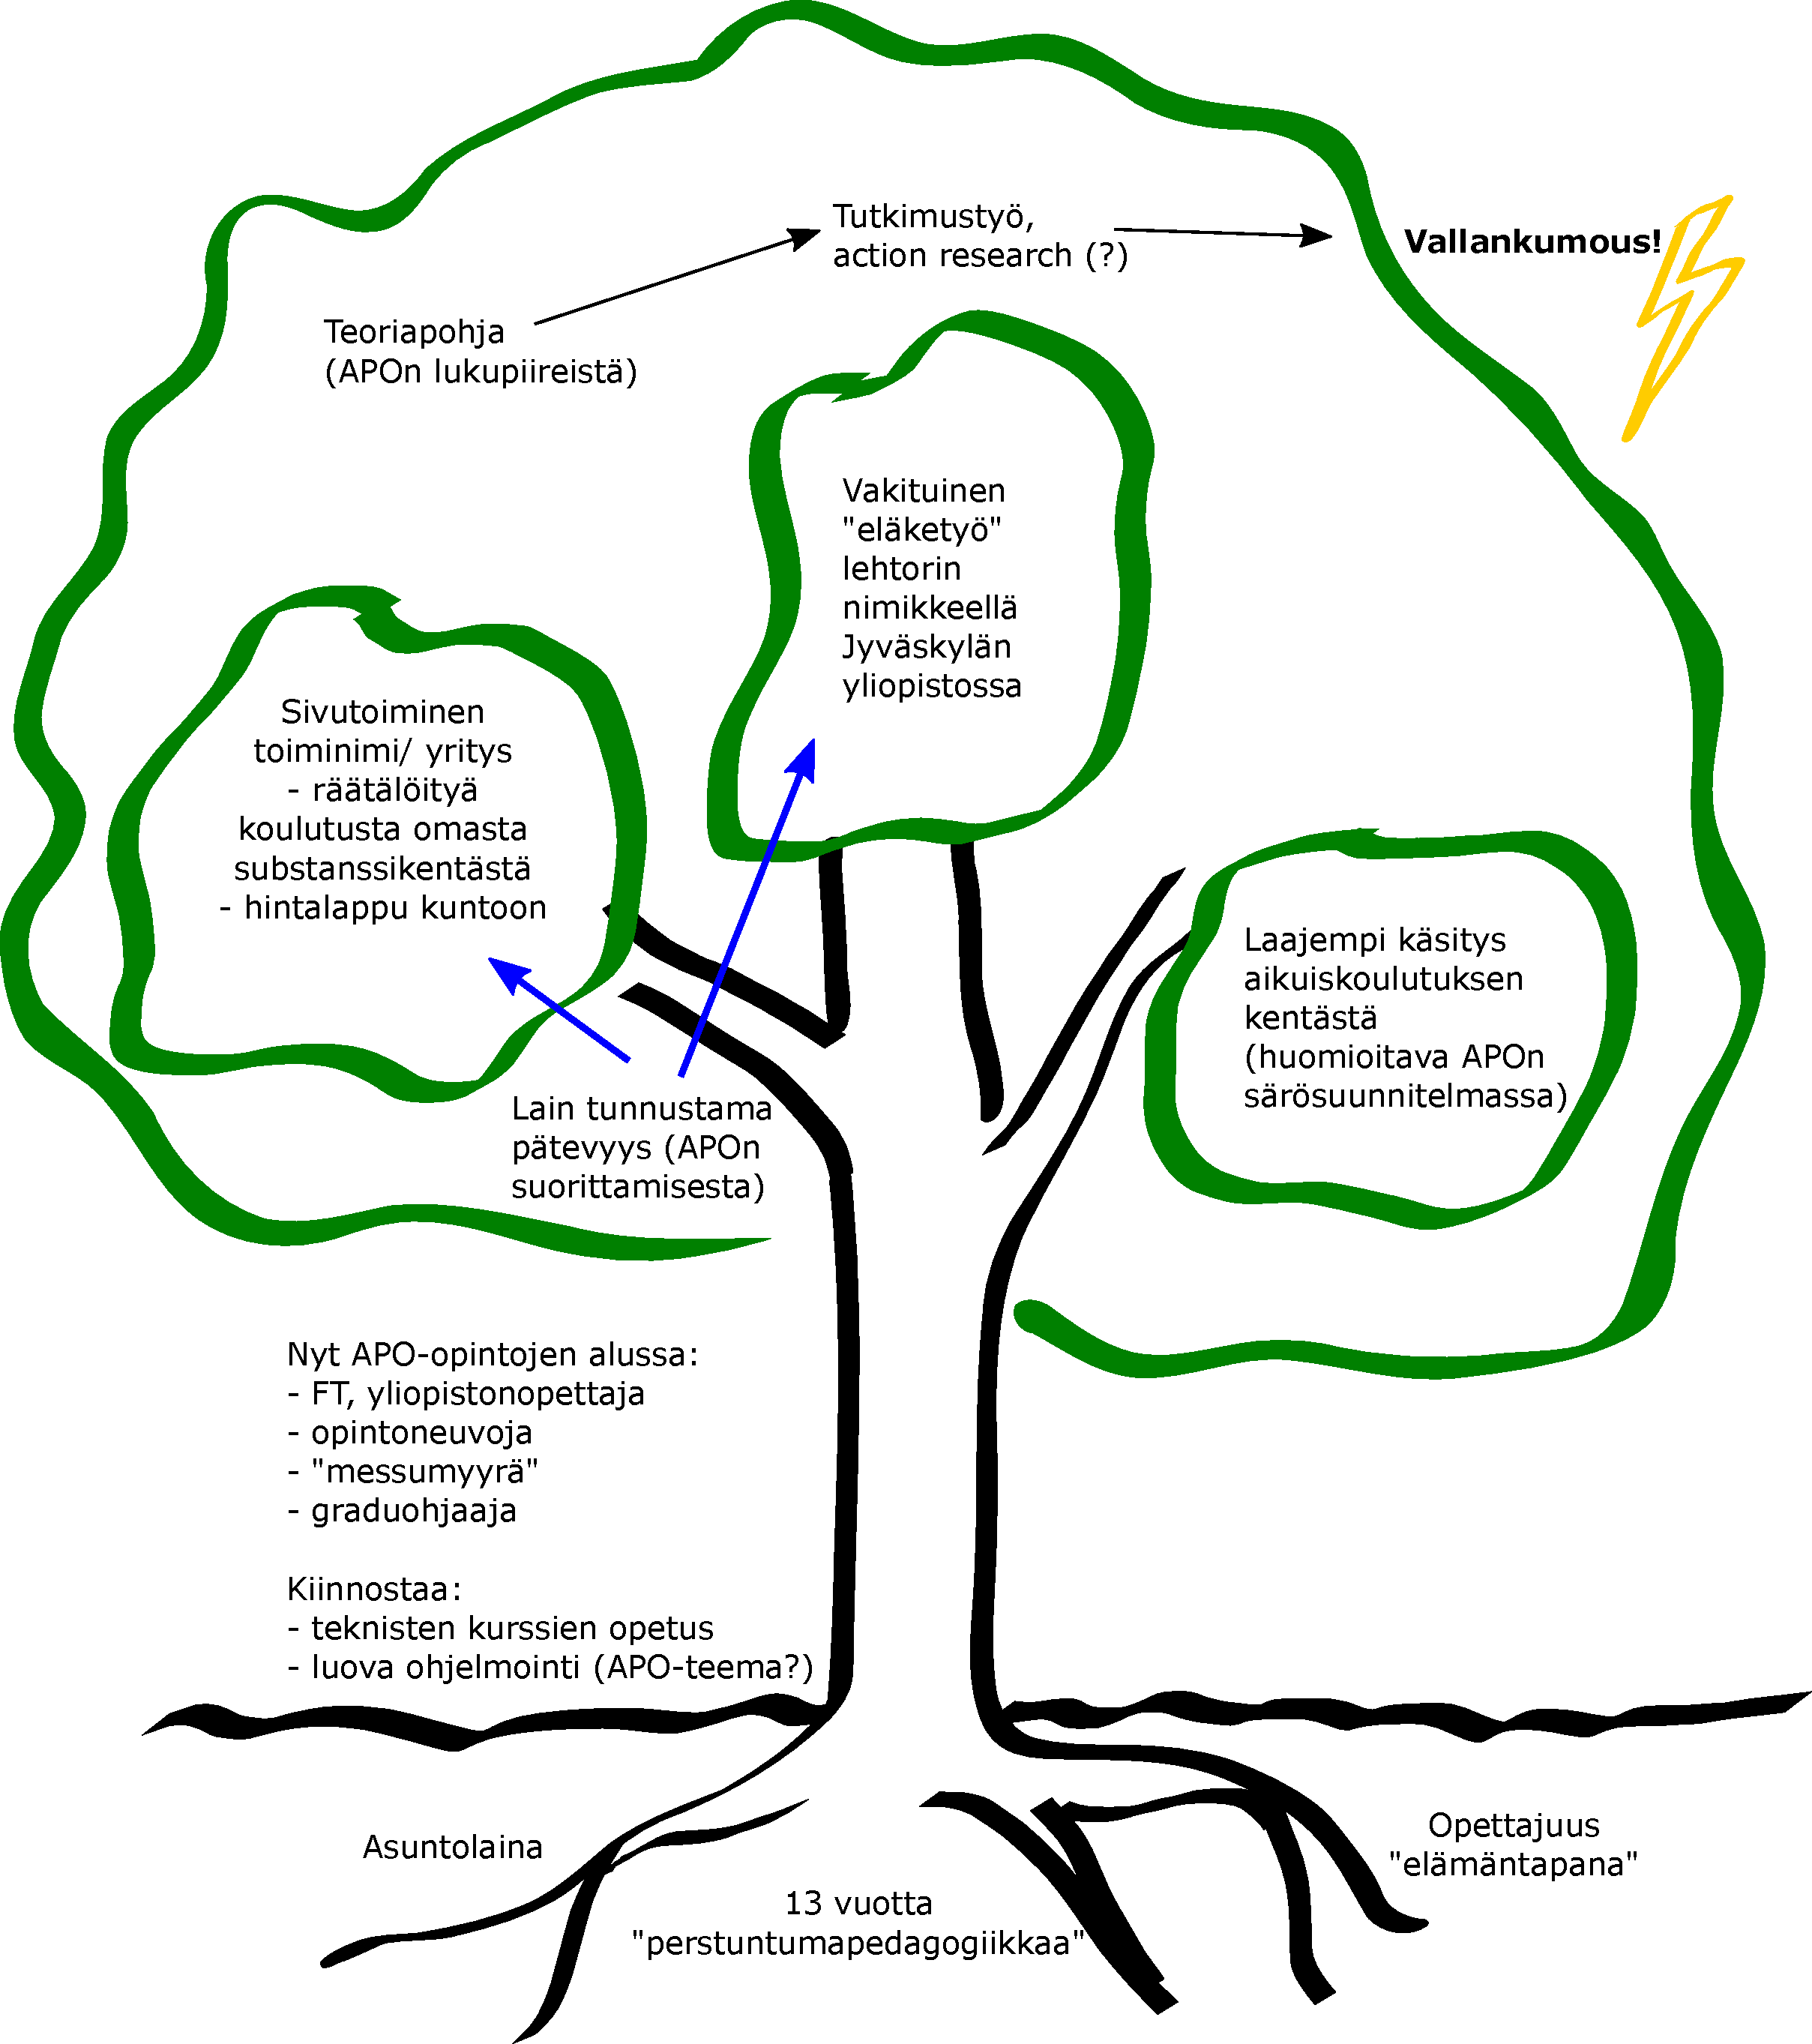
\includegraphics[width=.8\textwidth]{kaaviokuva}
  %
  % Ylläoleva koodi toimii sellaisenaan, jos tallennat kuvatiedostosi
  % PDF-muodossa tiedostoon nimeltä kaaviokuva.pdf esimerkkinä olleen kuvan
  % tilalle.
  %
  % Alla on normaali \label{tunniste} kohdassa, johon se kuuluu. Muuta
  % suomenkielinen otsikko vastaamaan oman kuvasi sisältöä.
  %
  \caption{\label{tekeleeni}APO-opintojen alussa piirtämäni tavoitepuu}
\end{figure}




\chapter{Pienin askelin kohti uusien taitojen oppimista}
\label{hopsJaGradu}

% Tämä teksti on jo kirjoitettu Oppimispäiväkirjan 3. osassa.
%
% LaTeXia varten se tarvitsee muutaman säädön:
%
%  - Alilukujen otsikot merkitään \section{Kuvaava otsikko}
%
%  - Jos on alialilukuja, ne merkitään \subsection{Kuvaava otsikko}
%
%  - Tehdään teknisesti kunnollinen viittaus luettuun graduun komennolla
%    \textcite{bibtexAvain} tai \parencite{bibtexAvain}.
%
%  - Prosenttimerkit ja muut LaTeX-kielen syntaksiin kuuluvat jutut pitää
%    laittaa jollain tavoin, minkä LaTeX ymmärtää (tai poistaa - less is
%    more:)).
%
%  - Suomalaiset lainausmerkit " on hyvä korvata kahdella heittomerkillä '' niin
%    tulee nätti.
%
%  - Tehdään muita pieniä säätöjä Markdownin ja LaTeXin syntaksien välillä.
%    Perusmallin esimerkkejä löytyy tekstini seasta:

Tämä luku jakautuu oppimispäiväkirjan 3. osan vaatimusten mukaisesti kolmeen
alilukuun. Ensimmäisessä on HOPSini perustelu, toisessa tiivistelmä lukemastani
gradusta ja kolmannessa pieni reflektio graduun liittyen.

\section{HOPSini sisältö ja perustelut}

Mikäs HOPS se minulla oikein on, kun en ole opiskelija ollenkaan? Tällä hetkellä
koen suorittaneeni formaalissa koulutuksessa kaiken tavoittelemani:
Tohtorintutkinnon ja aikuiskouluttajan pätevyyden kautta tie on nyt papereihin
leimatun koulutuksen osalta auki kaikkiin niihin hommiin, mitä tällä hetkellä
haaveilen tekeväni työkseni. Ja nyt ollaan humpsahdettu jo aiemmin
tavoittelemaani uraputkeenkin.

Mutta elämässä ei kannattane koskaan sanoa "ei koskaan". Paljonhan ilmeisesti
tapahtuu päähänpistoja, alanvaihtoja, toisia ja kolmansia väitöskirjoja eri
aloilta ja muuta. Ei ole vain itselleni tullut vielä tarvetta haaveiden
vaihdolle.

Akateemisessa työssä (ja nyky-yhteiskunnassa muuten monissa muissakin töissä!)
oppiminen, ja tavallaan siis opiskelu, myös jatkuu koko ajan --- tai sitten työn
tekijä on kyynistynyt valitettavalla tavalla ja on vaarassa pudota kelkasta
toimintaympäristön nopeassa muutoksessa. Tästä luvusta tuleekin esimerkinomainen
perustelu ''oikeaan HOPSiini'', vaikka sitä ei voi rakentaa ja aikatauluttaa
opintojaksolistana mihinkään opintotietojärjestelmään. Oppimispäiväkirjojen
kautta toivon opiskelijoidenkin etsivän nimenomaan ''oikeaa HOPSiaan'' eli
haaveisiin perustuvia osaamistavoitteita ja keinoja niiden saavuttamiseksi. Se
on paljon syvempi asia kuin OPSin mukainen lista kursseja HOPSissa!

Keväällä 2020 tuli maailmanlaajuinen yllätys koronaviruksesta. Me kaikki
joudumme nyt pakon edessä opettelemaan täydellisen etäopetuksen modaliteettia.
Se on vaikeaa ja hankalaa, kuten mikä tahansa uuden oppiminen. Pakko on aina
aivan hyvä peruste oppia, vaikkakaan ei yleensä miellyttävä. Mielenkiintoista on
se, että tämä tekstikappale on muuttunut syksyltä 2019 vain sillä tavalla, että
tässä oli silloin yllätyksenä ja pakko-opiskeluna opintotietojärjestelmä Sisu ja
nyt vuonna 2020 etäopetus. Minusta tämä on täydellinen esimerkki siitä, että
maailma muuttuu ja täällä joko opitaan muutoksen tuulien mukana tai pudotaan
kelkasta. Ja ainakin itse jotenkin nautin sitten siitä, kun yleensä sitten
selviytyykin muutoksesta, kun pystyy oppimaan ja mukautumaan. No se siitä\ldots\
HOPSiini kuuluu nyt Zoom, Skype, Teams, Moodle ja aivan uudenlaiset
toimintamallit, koska ne pitää oppia just nyt. Sisu oli (ja on edelleen)
valitettava ''ulkoinen motivaatio'' ja pakkopulla. Jotenkin sama luonnehdinta ei
päde etäopetuksen kohdalla\ldots\ olen aika pitkään haaveillut, että niin
sanotusti olisi aikaa opetella näitä juttuja. No ei aikaa ole nytkään, mutta
kaikki tämä, mitä nyt tulee, tuntuu tuovan kestävää hyötyä myös tulevalle ajalle
tämän vallitsevan kriisin jälkeen.

Tämä on nyt kolmas kerta, kun pidän tämän ITKY4000-orientaation. Paljon siitä,
mitä tulee, on vielä uutta. Otan tämän homman tutkivalla asenteella, avoimin
mielin, ja uskon oppivani paljon lisää, vaikka toki ensimmäinen kerta syksyllä
2019 opetti enemmän kuin mikään toisto nyt tai tulevaisuudessa. Ei ole olemassa
OPSia, jossa olisi valmiiksi ilmoitettuna lauseita, jotka alkavat sanoilla
''pidettyään ITKY4000-opintojakson, sen vastuuopettaja osaa\ldots '' vaan kyllä
minun piti selvittää se ihan itse syksyllä 2019, ja jatkan tässä harjoittelua
edelleen.

Toivon, että tämänkin ITKY4000-toteutuksen jälkeen ymmärrän aiempaa paremmin
niitä erilaisia tarpeita, joita ensimmäisen vuoden maisteriopiskelijalla on. Se
toivon mukaan kasvattaa kykyäni toimia myös OPSien kehittämistyössä, mikä aina
kolmen vuoden välein tulee eteen, viimeksi OPS-kautta 2020-2023 valmistellessa.
Tämän kolmannen kerran haasteena on kokeilla, toimisiko ITKY4000 koko
tiedekunnan yhteisenä toteutuksena. Aiemmin on ollut oppiainekohtaisesti
erilaiset toteutukset, ja kaikki on uutta ja hirmuisen jännää.

''Oikeassa HOPSissani'' työt ja harrastukset vyyhteytyvät toisiinsa: Haluan
kehittyä sekä opettajana että digitaalisessa taiteessa ja oman oppiaineeni,
tietotekniikan, perusasioiden käytännön ja teorian osaamisessa. Kiintopisteitä
ovat opintojaksot, joita pidän (Käyttöjärjestelmät, Tietokonegrafiikan
perusteet, Fysikaaliset mallit tietokoneanimaatioissa, tämä ITKY4000;
tulevaisuudessa mahdollisesti muitakin kursseja) sekä pääasiallinen
harrastukseni nykyään (demoscene). Uutena tekijänä on se, että tällä hetkellä
kartoitetaan resursseja Kääntäjätekniikan ja Ohjelmointikielten periaatteiden
opintojaksojen pitäjäksi. Minä en itse tiedä näistä asioista yhtään
mitään\ldots\ vielä. Mutta ryhdyin lukemaan kääntäjäoppikirjaa 3 sivun
vuorokausitahtia. Tätä kirjoittaessani on 50 sivua 1000:sta omaksuttu
harjoitustehtävineen. Jos tahti jatkuu, syksyllä 2021 pitäisi alkaa olla tieto-
ja taitopohja alustavasti kunnossa myös aiheen opettamiseen.

Tällä hetkellä opiskelen harrastuksena myös Forth-ohjelmointikieltä ja siihen
liittyvää ajattelua. Konkreettinen tavoitteeni oli osallistua jo Assembly Summer
2020 -tapahtumassa ''4k intro'' -kilpailuun (se on siis audiovisuaalinen
taidetuotos, joka pitää toimittaa korkeintaan 4096 tavun mittaisena
suoritettavana ohjelmatiedostona) kokonaan Forth 2012 -standardin mukaisena
lähdekoodina tehdyllä tuotoksella, joka käynnistyy AMD64-konekielellä itse
tekemäni Forth-tulkin päällä. Samalla tuotan omasta mielestäni kovin
esimerkillistä oppimispäiväkirjaa / tuntikirjanpitoa, jonka voin jatkossa
näyttää konkreettisena esimerkkinä jonkin itsenäisesti suoritettavan
opintojakson palautusmuodosta. Tartuin toimeen elokuussa 2019, takana on nyt 300
tuntia eli reilun 10 opintopisteen verran itseopiskelua. Korona sotki
alkuperäiset aikataulusuunnitelmat, mutta lähivuosina näyttäisi suurella
varmuudella tulevan kohtalaisen härö tuotos ulos. Ohjelmointikielet, tulkit ja
kääntäjätekniikka rupesivat tekemisen kautta kiinnostamaan tosi paljon, ja olen
alkanut esimerkkien kautta tutustua myös Lisp-kielen toteuttamiseen C:llä.

Demoscenetapahtumissa on varmasti jatkossakin ohjelmointityöpajoja, joita olen
tehnyt harrastuksena talkootyönä. Siitäkin harrastuksesta koetan ammentaa lisää
harjaantumista opettajana.

Millainen vyyhti? Kun silmäilen äsken kirjoittamiani konkreettisia harjoituksia
eli tämän vuoden opintosuunnitelmaani ja aikataulua, niin voin todeta sen olevan
linjassa päämäärieni ja kiintopisteideni kanssa. Tekemisessä ei näytä olevan
rönsyjä suuntiin, joiden avainsanat eivät löytyisi tavoiteasettelusta. Eli hyvä
vyyhti vaikuttaisi olevan, ja se on jaettu konkreettisiin, nykyisistä
pohjatiedoista lähtien toteutettavissa oleviin välietappeihin, joista kertyy
todennettavissa olevaa portfoliota --- julkaisuja, jotka jäävät olemaan ja
joiden alkeellisuudelle voi itsekin naureskella vuosien päästä, kun on oppinut
taas lisää.

Perille ei muuten sitten pääse yhdessä oppimispäiväkirjamerkinnässä, eikä
pidäkään! Itse olen miettinyt näitä asioita vuosikausia ja kirjoittanut aika
ajoin HOPSeja milloin missäkin yhteydessä. Ei siis haittaa, vaikka vielä
ITKY4000:ssa opiskelijan ajatukset ovat enemmän hajallaan tai päämäärät
epäselviä. Tärkeintä on viimeistään tässä vaiheessa \emph{aloittaa} niiden
pohtiminen ja kirjoittaminen auki! Ensin on raapaistava pintaa, että koskaan
pääsisi syvemmälle. Sanoittamatta jäänyt haave on isossa riskissä jäädä
toteutumatta, ja ilman selkeää päämäärää on aika vaikea keksiä, mihin suuntaan
seuraava askel pitäisi ottaa.



\section{Gradu, johon tutustuin}

Päätin käsitellä tässä Esa Hiivan vuonna 2018 kirjoittamaa gradua
''Virtuaalitodellisuuspelien tilavaatimuksien pienentäminen kotikäytössä
uudelleensuunnatun kävelyn avulla'' \parencite{Hiiva2018vr}. Olen muuten saanut
häneltä henkilökohtaisesti luvan käyttää gradua esimerkkinä tässä!

\subsection{Miksi valitsin juuri tämän}

Perustelen tekemääni graduvalintaa useammallakin seikalla. Tärkein syy on se,
että olemme jatkaneet tekijän kanssa työtä aiheen parissa. Esa on valmistumisen
jälkeen siirtynyt jo muualle, mutta hän on ''siviilitutkijana'' tiivistänyt ja
kääntänyt gradunsa sisältöä englanniksi ja olemme pitkällä projektissamme saada
gradussa tehty tutkimus tieteellisen artikkelin muotoon ja vertaisarvioitavaksi
kansainväliseen tiedelehteen. Kuinka ollakaan, COVID-19 sotki aikataulut
tämänkin osalta, mutta tilanne on edelleen toiveikas. Ei ole aivan tavanomainen
asia, vaan melko harvoin eteen tuleva mahdollisuus julkaista gradun tuloksia
kansainväliselle tiedeyhteisölle. Myöskään ei ole missään nimessä tarkoitus,
että keskimääräinen, sananmukaisesti \emph{hyvä} gradu, sisältäisi vastaavaa
julkaisupotentiaalia. Esimerkin ja ideaalin tavoitepisteen tämä kuitenkin
asettaa, koska mikä onkaan aina sen vahvempi osoitus tiedekunnan kyvystä tarjota
tutkimukseen perustuvaa ylintä opetusta kuin se, että opinnäytteet tuottavat
todisteellisesti kansainvälisesti relevantteja tutkimustuloksia! Gradujen tason
nosto nykyistä enemmän julkaisutasoisiksi onkin ensisijainen päämääräni, jonka
nostin lippusalkoon työhakemuksessani nykyiseen yliopistonlehtorin työhöni.

Muitakin graduihin perustuvia julkaisuprosesseja on työn alla, mutta omien
ohjausteni pohjalta lähteneiden osalta Esan työ on ehtinyt tähän päivään
mennessä pisimmälle, mistä syystä oli helppo napata tähän esimerkiksi juuri se.
Osasyy valintaan on sekin, että minun ei tarvinnut käyttää ylimääräistä aikaa
lukemiseen, koska tämä kyseinen gradu on pysynyt viikottain mielessä aina
valmistumisestaan asti.

Lienee perusteltua yksilöidä orientaatio-opintojakson esimerkkiin juuri
tällainen erinomainen opinnäyte. Maisteriopiskelijan on kuitenkin hyvä tutustua
myös tyypillisempiin graduihin. Tässä oppimispäiväkirjassa aloitetaan yhdestä
gradusta ja opitaan samalla löytämään lisää esimerkkejä
JyX-julkaisujärjestelmästä. Harjoitteita jatketaan myöhemmin
seminaariopintojaksolla, mutta pidän tärkeänä orientoitua opinnäytteeseen alusta
asti.

\subsection{Objektiivinen sisältökuvaus}

\textcite{Hiiva2018vr}
etsii keinoja huonemittakaavan virtuaalitodellisuuspelien tilavaatimusten
pienentämiseen kotikäytössä. Teoriakatsaus alkaa virtuaalitodellisuuden (VR)
yleiskuvauksesta ja etenee kuvailemaan gradun nimenomaista aihepiiriä eli
tapoja, joilla VR:n käyttäjä voi liikkua virtuaalimaailmassa paikasta toiseen.
Erityisenä kiinnostuksen kohteena on luonnollinen kävely, jossa kotikäyttäjä
kävelee silmikko päässään esimerkiksi olohuoneessaan, johon on tehty tilaa
huonekaluja siirtämällä. Saatavilla olevien käyttötilastojen mukaan nämä tilat
ovat yleensä aika pieniä pinta-alaltaan. Gradun keskiössä on kysymys siitä,
miten tilatarvetta voidaan vähentää erityisesti manipuloidun kävelyn avulla.

Manipuloitu kävely tarkoittaa yksinkertaisimmillaan sitä, että yhden metrin
kävely olohuoneessa näyttääkin virtuaalitodellisuudessa kahden metrin
mittaiselta. Myös suuntaa voidaan manipuloida: 180 asteen käännös olohuoneessa
voikin näyttäytyä virtuaalimaailmassa kokonaiselta 360 asteen kierrokselta.
Liian suuri tai vääränlainen manipulointi johtaa siihen, että kokemus ei tunnu
enää riittävän aidolta, ja pahimmillaan käyttäjälle voi aiheutua jopa
pitkäkestoista pahoinvointia.

Hiiva kehitti gradussaan kaksi uutta paikannuslaitteen käyttöön perustuvaa
manipuloidun kävelyn menetelmää VR-ympäristössä. Näitä ja valittua
verrokkimenetelmää sekä menetelmien aiheuttamaa simulointipahoinvointia
arvioitiin niin sanotulla parivertailumenetelmällä sekä paperisin kyselyin 19
koehenkilön otannalla.

Empiirisessä osiossa Hiiva rakenteli Unreal Engine 4 -pelimoottorilla pienen
testipelin käyttäjätutkimuksen koeasetelmaksi. Sitten hän teetti 19
koekäyttäjällä testin ja analysoi tulokset parivertailumenetelmän mukaisesti.
Empiiristen osioiden yhteyteen on kirjattu myös useita käytännön vinkkejä
manipulointimenetelmiä käyttävien VR-pelien kenttäsuunnitteluun.

Johtopäätöksenä tarvittavan fyysisen tilan kokoa pystyttiin pienentämään
käyttäjätestiin valikoituneilla menetelmillä noin kolmanneksella, ja käyttäjät
pitivät näitä menetelmiä mielekkäinä liikkumismuotoina VR-pelissä.


\subsection{Ajatuksia, joita lukuharjoitus herätti}

Tässä kannattanee vielä kerran korostaa sitä, että Hiivan gradu oli
poikkeuksellisen laaja ja isotöinen. Tyypillisempää ja \emph{riittävää} hyvään
arvosanaan olisi näppituntumalta noin puolet tästä kyseisestä gradusta (ainakin
tietotekniikan oppiaineessa; en itse pysty ottamaan kantaa muihin
oppiaineisiimme). Tällainen siitä nyt lopulta tuli
%
käsittääkseni sitä kautta, että tekijällä oli itse valitsemaansa aihepiiriin
omakohtainen kiinnostus ja ''polte'', joka pisti tekemään ja jaksamaan enemmän
kuin niin sanotusti vaaditaan. Lisäksi käytetyt laitteistot ja
ohjelmistolisenssit olivat suurimmalta osin tekijän itse hankkimia.

Ohjaajana on valtavan hienoa nähdä, kun tällainen innostus silloin tällöin
syttyy. Opettajana on houkuttelevaa kuvitella mielessään, että on ehkä jollakin
vuosien takaisella opintojaksolla kenties saanut heiteltyä sytykkeitä, jotka
sitten ajan mittaan roihahtavat kiinnostuksen paloksi (se on siis kuvitelma,
joka auttaa itseäni jaksamaan; en tiedä, oliko vaikkapa pitämälläni grafiikan
peruskurssilla mitään osaa taikka arpaa tähän kyseiseen lopputulemaan; illuusion
suojelemiseksi tulen myös olemaan kysymättä asiasta).

Informaatioteknologian graduohjeet löytyvät Internetistä%
\footnote{\url{https://www.jyu.fi/it/fi/ohjeita-opiskelijalle/opiskelu/pro-gradu-tutkielma}}.
%
Kriteerit ovat tällä hetkellä eri oppiaineissa erilaiset. Tässä esimerkissäni
käytän tietotekniikan gradujen arvosteluohjetta%
\footnote{\url{https://www.jyu.fi/it/fi/ohjeita-opiskelijalle/opiskelu/pro-gradu-tutkielma/tietotekniikka/gradun-arvosteluohjeet}}.
%
Käsitykseni mukaan koulutusteknologia käyttää tällä hetkellä (18.9.2020) vielä
samaa kriteeristöä kuin tietotekniikka.
%
Tietojärjestelmätieteen, kyberturvallisuuden ja kognitiotieteen arvosteluohje%
\footnote{\url{https://www.jyu.fi/it/fi/ohjeita-opiskelijalle/opiskelu/pro-gradu-tutkielma/tjt-kyber-kog/gradun-arvostelukriteerit}}
on hieman erilainen.
%
Omaa oppimispäiväkirjaasi varten varmista, mikä on oman oppiaineesi kriteeristö
gradun arvioinnissa. Käytä kyseisiä ohjeita ja valitse JyXistä juuri oman
oppiaineen gradu tarkasteltavaksesi.

Menemättä tässä ja lupaa kysymättä sinänsä ei-julkiseen arviointilausuntoon
Hiivan gradun osalta, voin luonnehtia työtä omasta mielestäni
''esimerkilliseksi'' useiden ohjelmisto- ja tietoliikennetekniikan gradun
tärkeimpien kriteerien suhteen.

Aina jää parantamisen varaakin. On esimerkiksi osa kaaviokuvista ärsyttävästi
rasterigrafiikkana, minkä jouduimme korjaamaan kovalla työllä sitten jälkikäteen
julkaisua varten\ldots\ Jo tekemisen aikana oltaisiin selvitty huomattavan
paljon pienemmällä vaivalla, jos \LaTeX -ladontajärjestelmä olisi ollut
prosessin alusta lähtien käytössä. Myös siirtäminen oikean tieteellisen lehden
\LaTeX -pohjaan olisi ollut ''copy-paste-modify'' -toimenpide, mutta nyt täytyi
rakentaa paljon uusiksi jälkikäteen. Onneksi nämä hankaluudet eivät ole enää
minkäänlaisia tekijöitä tulevissa tietotekniikan graduissamme, koska heti
ITKY4000-opintojaksolla tietotekniikan opiskelijat opettelevat niistä eroon ja
tulevaisuudessa voidaan vaan unohtaa moisten ongelmien olemassaolo tykkänään!
Tietotekniikan taitaja kun voi ja hänen pitäisi! (Muiden oppiaineiden eli KOG,
KOTE, KYB, TJT, TSAMO opintoneuvojat saavat antaa halutessaan erilaiset ohjeet
oppimispäiväkirjan 4. osaan:))

Se käynee kelle tahansa lukijalle ilmiselväksi, että \textcite{Hiiva2018vr}
perustelee gradussaan jotakuinkin kaikki ratkaisut ja lausumat joko omaan
empiiriseen aineistoon tai aiempaan akateemiseen tutkimukseen vedoten, jota on
myös etsitty, luettu, ymmärretty ja sovellettu laajasti. Tärkeimpiä vahvuuksia
ovat:

\begin{itemize}
\item tutkimuskysymyksen perusteleminen ajankohtaiseksi aiempaan tieteelliseen
  tutkimukseen objektiivisesti vedoten sekä

\item tarkoituksenmukaisen, maailmalla hyväksi havaitun, tutkimusmenetelmän
  valinta.
\end{itemize}

Nämä asiat kun on kunnossa, niin ollaan jo pitkällä minkä tahansa tutkimuksen
tekemisessä!

Vaikka koen tarpeelliseksi nostaa esimerkin tällaisesta ''ideaaliprosessista'',
en haluaisi että kukaan ryhtyy stressaamaan siitä, ettei ole vielä esimerkiksi
löytänyt erityistä innostuksen kohdetta tai kiintopistettä alalta. Sitähän voi
joutua etsimään vaikka useamman tutkinnon ja työelämävuosien ajan! Kaikki
tiedämme, että se on elämässä ihan normaalia kaikkien osa-alueiden kohdalla.

Etsiminen ja pohtiminen ei kuitenkaan voi koskaan haitata mahdollisuutta löytää
jotakin, ja\ldots\ siksipä tässä tehdäänkin juuri tällaista
ITKY4000-opintojaksoa ja tällaista Oppimispäiväkirjaa kaikkine pohdintoineen.
\emph{Trust me - I know what You should be doing.} Itselleni tärkein ajatus
tämän esimerkin viimeistä lausetta kirjoittaessa olikin aikoinaan, että olin
entistä varmempi, että tämän tehtävänannon kautta ITKY4000 kulkee juuri oikeaan
suuntaan. Olen samaa mieltä yhä syksyllä 2020, jatkuvan itsekriittisen
tarkastelun jälkeenkin ja varsinkin luettuani yli 100 oppimispäiväkirjaa, joiden
osana oli oman oppiaineen gradun kriittinen lukeminen ja siitä heräävien
tunteiden kirjaaminen!

% ------------------------------------------------------------------
%
% Tähän asti tuli muokkaamalla ja täydentämällä oppimispäiväkirjan osia 1-3.
% Seuraavaksi on 4. osan loppupohdinnan paikka.
%
% Korvaa esimerkit aliotsikoiden alta oman pohdintasi mukaisiksi.
%
% ------------------------------------------------------------------

\chapter{Katse kohti tulevaa nykypäivän kautta}
\label{muitaAsioita}

Tässä luvussa on neljä pakollista alilukua, joihin kirjoitetaan uutta:
Ensimmäiseen tulee yliopiston jokaiselta tutkinto-opiskelijalta edellyttämä
kansainvälistymissuunnitelma. Toiseen alilukuun tehdään itsearvio opiskelun,
oppimisen ja muun elämän sujumisesta ITKY4000-opintojakson alkamishetkestä tähän
päivään asti, kolmannessa koetetaan keksiä parannuksia tulevaisuutta varten, ja
neljännessä mietitään erityisesti ITKY4000:n roolia.

\section{Kansainvälistymissuunnitelmani}

\textit{Tehtävänanto: Kuvaile, millä tavoin olet suunnitellut huomioivasi
  opintojen aikana kansainvälistymisen näkökohtia. Tällä tarkoitetaan
  kaikenlaista valmistautumista modernissa tietotyössä mahdollisesti
  kohdattavaan kulttuurien monimuotoisuuteen sekä kommunikaation ja
  verkostoitumisen kehittämisen rajojen yli.}

Minua jäi aikoinaan harmittamaan kovasti, että en joko uskaltanut tai saanut
aikaan lähteä opiskelijavaihtoon kandi- tai maisteriopintojeni aikana. Itselleni
annoin syyksi parisuhteen sekä kiinteät työt ja harrastukset. Jälkikäteen pidän
niitä kuitenkin tekosyinä, joilla peittelin jotakin ärsyttävämpää,
tiedostamatonta, peikkoa. Ohjaamiani opiskelijoita olen sitten koettanut
rohkaista ja tukea ajatuksissaan vaihdosta, ja moni on kiitellyt jälkeenpäin
pienestä tönäisystä tärkeään ja joskus elämää muuttavaan vaihtokokemukseen.
Tässä se nyt taas tulee: tee itsellesi palvelus ja pohdi perusteluineen
nykyisessä tilanteessa mahdollisuuksia työ- tai opiskeluvaihtoon, varsinkin jos
sellaista ei vielä historiastasi löydy.

Jos vaihto ei ole realistinen tai ei jostain syystä toteudu, mahdollisuutena on
myös kotikansainvälistyminen, mitä olen sitten itse aika onnistuneesti
harrastanut. Erityisesti Jyväskylässä on kesäisin kansainvälinen kesäkoulu
Jyväskylä Summer School, joka on paikallisille opiskelijoille ilmainen. Sen
opetus on syventävän tasoista, ja informaatioteknologia-aiheiset opintopisteet
käyvät suoraan osaksi syventäviä maisteriopintoja (ja itselläni aikoinaan
jatko-opintojen kursseiksi).
%
Monet kesäkouluissa syntyneet kansainväliset kontaktit ovat jääneet pysyviksi,
ja jotenkin tässä on sitten saanut kokemuksia väitöstilaisuudesta Trondheimissa,
perhepääsiäisestä Prudnikissa, uudenvuodenjuhlasta Tbilisissä ja Volgan
rannoista Jaroslavlissa. Kertaalleen tuli myös kolmen viikon Interraililla
käytyä läpi Euroopan keskeisten opiskelijalähiöiden opiskelija-asuntolat ja
niiden lähibaarien happy hour -valikoimat.
%
Ensitapaamisen kontekstista johtuen kaveriverkosto alkaa nyttemmin olla
merkittävissä positioissa tiede- ja teknologiabisneksessä ympäri maailmaa, mikä
voi kait joskus osoittautua hyödylliseksi. Että hoitui se kansainvälinen
verkosto näköjään noinkin, mikä vähän hälventää kismitystä siitä, että vaihto
jäi itseltä väliin aikanaan.

Nykyinen työ on sitten luonnostaan kansainvälistä, kun työkaverit ovat kuka
mistäkin päin maailmaa. Tiedehommissa on päässyt useampaan otteeseen
konferensseihin, joissa verkostoa on mahdollista päivittää.
Konferenssi-illallisen jatkoilla taidettiin alunperin tutustua myöhemmin
toteutuneen akatemiahankkeen ulkomaisiin partnereihin. Ei pidä aliarvioida
kasvotusten tapahtuvan kommunikaation ja yhteisen vapaa-ajan viettämisen roolia
työhönkään liittyvien verkostojen syntymisessä, niin kotimaassa kuin
kansainvälisesti.

Joka tapauksessa kansainvälistyminen tavalla tai toisella on nykyään tärkeää, ja
kehotan miettimään mahdollisia strategioita omalta kohdalta, itselle
sopivimmilla tavoilla. Siksipä kansainvälistymisen suunnittelu on omalla
vahtivuorollani ollut ITKY4000:n OPSissa ja alusta lähtien oppimispäiväkirjan
vapaaehtoisena lisätehtävänä. Yliopiston linjauksetkin tulivat sittemmin ajan
tasalle, jolloin tämä osio oli helppo vain siirtää vapaaehtoisesta pakolliseksi
osioksi.

\section{Itsearvio syksystä 2019}

Esimerkin lukija huomatkoon, että tätä lukua ei voi kirjoittaa ennen kuin
lukukausi on loppukatsausta vaille valmis. Mikäli joskus on aikaa päivittää
esimerkki, teen sen. Enpä kuitenkaan pidättele hengitystäni ajan löytymisen
suhteen. Ainakaan vielä syksyn 2019 jälkeen sitä hetkeä ei ole ehtinyt tulla.
Esimerkkinä tämä kuitenkin toiminee yhtä hyvin kuin kirjoitushetkellänsä
aikoinaan. Eläytykäämme aikaan vuosia ennen koronaa, kun Sisu oli juuri otettu
käyttöön.

Olipahan hommaa tässä syksyssä [2019] ja sitähän vielä vähän jatkuukin. Kiire ja
rästihommien kertyminen ovat jääneet syksystä päällimmäisenä mieleen ja lisäksi
Sisun käyttöönoton aiheuttama päivittäinen järjestelmävitutus.
%
Mukautumista olosuhteisiin on joutunut tekemään ja työn tulosten
keskeneräisyyttä sietämään enemmän kuin yleensä.
%
Se on ehkä positiivista huomata jälleen kerran, että kaikenlaiseen taipumiseen
ja venymiseen pystyy tarpeen tullen.
%
Mutta kyllä myös väsymyksen huomaa, ja tekeminen on tuntunut monin paikoin
epämiellyttävältä ihan päivien pituuden vuoksi. Sitä alkaa olla vähän niinkuin
loman tarpeessa ihminen tässä.

Onneksi marraskuussa ei tarvitse opettaa mitään opintojaksoa, joten kalenterissa
on toistaiseksi melko väljän näköistä ennen joulukuussa todennäköisesti
odottavaa valmistumisten ja graduviimeistelyjen ruuhkaa. Ja tammikuusta
kesäkuuhun on sitten ehkä vielä kovempi ruuhka [ja tämähän oli kirjoitettu ennen
kuin COVID-19 osui siihen kuuluisaan tuulettimeen]. Tosi paljon toivon, että
ohjelmisto- ja tietoliikennetekniikan maisteriopintoneuvontaan löytyy apukäsiä
ennen tammikuuta.

Oppimisen saralla tässä ei mitään mullistavia läpimurtoja tunnu nyt tapahtuneen.
Tuli ajankohtaiseksi oppia laittamaan Moodleen juttuja, editoimaan videoita,
tekemään pieniä opetusvideoita ja pitämään etäsessioita. Nämä ovat pitkälti
kuitenkin teknisiä yksityiskohtia, jotka eivät tuo uutta osaamista tai
ymmärrystä. Kaikki on aina vaan KVG, ja kun osaa KVG:n niin juurikaan uusia
haasteita ei tule.
%
Onhan se aina voimaannuttavaakin saada käyttöön joku uusi työkalu tai menettely
ja aistia sen valtavat mahdollisuudet. Mutta sitten tarvitsisi aikaa kokeilla
sillä jotakin uutta ja luovaa, ja aikaa ei nyt ole ulkoisten syiden vuoksi. Se
hieman lannistaa. Mutta optimistina luotan, että kyllä tämä vielä tästä
helpottaa ja ehdin mennä syvemmälle kaikkiin noihin juttuihin joskus.

Oikean HOPSini mukaiset harrastusprojektit ovat olleet käytännössä täysin
pysähdyksissä, joten niiden osalta ei ole edes mitään arvioitavaa. Ai niin,
paitsi että aloitin Linkki Jyväskylä ry:n myötävaikutuksesta lyhyesti uuden
harrastuksen, josta tulee vielä suosikkini myös grafiikkakurssien opettajana.
Vasta pari tuntia ehdin treenata Shader Showdownia eli livevarjostinkoodausta
GLSL:llä, mutta ne olivat pari tosi voimaannuttavaa tuntia. Näytösottelua Linkin
laneille en saanut järjestettyä, koska osasin kerrankin kieltäytyä
ylimääräisistä viikonloppuaktiviteeteista. Ehkä mulla on siis toivoa myös sen
kestohaasteeni eli ajankäytön hallinnan osalta. Kieltäytyminen ja omien rajojen
asettaminen ajankäytössä siinä varmasti on tosi tärkeä (ja itselleni tosi
vaikea) asia. Ja toiminnan kalenterointi ja kalenterissa pysyminen. Kyllä tässä
syksyssä on ollut valonpilkahduksia tämän osalta: kalenteriin ennalta merkityt
tyhjäkäyntiajat ovat muistaakseni paljolti pysyneet tyhjäkäyntinä, minun ja
vaimon yhteisinä hengähdyshetkinä.



\section{Miten kehitän toimintaani jatkossa}

Otsikon mukainen kysymys on tärkeä miettiä läpi usein.  Tarkoitus olisi nyt
peilata syksyä ja edellisessä kohdassa tehtyä itsearviota miettien, että voisiko
heikosti menneitä asioita joillain keinoin tehdä jatkossa paremmin. Tämän
ulkoisista syistä hiukan Sisuttaneen syksyn osalta siihen on vähän vaikea
vastata. Kysymys olisi kuitenkin oman toiminnan parantamisesta ja muista
asioista, joihin voi itse vaikuttaa. Omaan toimintaan liittyvä ratkaisu ei
oikein voi olla yliopiston opintotietojärjestelmän vaihtaminen tai edes
käyttämättä jättäminen.

Heikoimmin itselläni menee nyt monetta vuotta putkeen ajankäytön hallinta ja
omasta hyvinvoinnista huolehtiminen. Toiveissa oli kaikessa rauhassa miettiä ja
kokeilla jotakin uusia keinoja aiheen parissa tänä syksynä. Nyt tuli toki
mietittyä ja kokeiltua, mutta varsin hätäisesti ja ajattelua ehkäisevän kiireen
keskellä. Silti jotain saattoi löytyäkin\ldots\ konkreettisena menettelynä, jota
aion käyttää jatkossa ovat HOPS-päivystykset mikroluokassa. Ne vaikuttavat
olevan hyvin moneen HOPSin ylläpitokysymykseen aivan riittävä tilaisuus, ja
resurssitehokkuudessaan verraton.
%
Ryhmäohjauksia on ollut visioissa hyödyntää myös omien graduohjausten
tehostamiseen, mutta tämä syksy ei mitenkään ole mahdollistanut uusia kokeiluja
sillä puolen kenttää.

Kalenterointia, varsinkin tyhjäkäyntiin ja rentoutumiseen varatun ajan
kalenterointia, pitää opetella lisää. Jatkuvana haasteena on osata sanoa se
''ei'' useammin ja jättää sinne kalenteriin oikeata ''tässä ei tapahdu tasan
mitään'' -aikaa. No niin. Löytyihän sieltä kaikkein kriittisimmät asiat. Nämä
muutamat jos saisi kuntoon niin voisi miettiä jotakin seuraavia, pienempiä,
kehityskohteita. Eivät ole helppoja, mutta minä toivon että nyt kun ainakin
tiedostan nämä kehityskohteet niin ehkä niissä on joskus vielä mahdollista
jotenkin päästä eteenpäin, kun päivittäin koettaa harjoitella.

\section{Mitä ITKY4000 ja tämä oppimispäiväkirja antoivat minulle}

Tähän kohtaan toivon opiskelijan kirjoittavan avoimesti ja omin sanoin tämän
hetkisiä omia mietteitään siitä, mitä otsikko herättää suhteessa tällä
ITKY4000-toteutuksella tapahtuneeseen eli vapaaehtoiseen tapaamistarjontaan ja
pakollisina palautustehtävinä suoritettaviin oppimispäiväkirjoihin.
%
Toivon, että pohdinta jollain tapaa sulkee ympyrän, joka ensimmäisessä
oppimiskirjassa pohdituista kysymyksistä alussa lähti piirtymään.
%
Maisteriopinnot jatkuvat silmukan seuraavaan kierrokseen, mutta mielestäni
jokaisen kierroksen jälkeen on hyvä katsoa taaksepäin, että voi ottaa suuntaa
eteenpäin.
%
Jokainen kirjoittakoon itseään varten, vaikka tietäisi että opettaja lukee.
Jälleen teen esimerkillisesti samoin itse, vaikka tiedän että opiskelija lukee
(tai ainakin toivottavasti hiukkasen tarkastelee tätä tehtävän esimerkkinä
annettua pohjaa).


Aloitan siitä, mitä tämä oppimispäiväkirja minulle antoi. Sehän antoi lähinnä
teknistä lisätyötä, koska päiväkirjan ja muiden dokumenttien kirjoittaminen on
päivittäistä rutiinipuuhaa muutenkin, eikä näissä pohdinnoissa nyt ollut
mahdollista päästä kummempiin läpimurtoihin sen jälkeen, mitä APOssa
kirjoitettiin ja kaiveltiin läpi vuoden ajan.
%
Ja vaikka tämä on kaikki rehellistä, niin kertomatta jää henkilökohtaisimmat
asiat, jotka siellä aivan omassa ja salaisessa päiväkirjassa voivat olla
kaikkein tärkeimmät avaimet kohti ratkaisuja.
%
Mielestäni näistä nyt tuli desinfioituinakin tarkoituksenmukaiset esimerkit
ITKY4000-opintojaksolle, ja toivon, että joku ehkä vähän harvemmin
oppimispäiväkirjoja tehnyt löytää tällaisten tekemisestä uutuuden viehätystä ja
konkreettista hyötyä tulevaisuuttaan kohti.


Entäs tämä ITKY4000? Opintojakson pitäminen tuntui hyvin kaukaiselta ja
vieroksuttavalta ajatukselta siinä vaiheessa, kun minua pyydettiin tätä pitämään
jossain vaiheessa kesää 2019. Silloinkin oli hyvin ruuhkainen aika ja olin
opettelemassa kieltäytymistä kaikenlaisesta ja erityisesti kaikesta, mikä on
uutta nykyisen kuorman päälle.
%
Otin kuitenkin nakkihomman vastaan, kun ei siinä tainnut muitakaan juuri olla
käytettävissä ja myös halusin, että ITKY4000 hoituu niiden kohtalaisen jaloina
pitämieni pedagogisten periaatteiden mukaan, joita sen arkipäiväisen nimen
takana on pohdittu kahvihuoneissa ja OPS-työryhmissä vuosikausien ajan.
%
Ratkaisuun vaikutti varmasti sekin, että ITKY4000 tarjoaisi mahtavan
mahdollisuuden kokeilla kaikkea APOssa juuri edellisenä vuonna oppimaani
käytännössä.


OPS-suunnittelun lisäksi olen ollut ITKY4000-opintojakson kanssa aiemmin
tekemisissä vain HOPS-ohjaajan roolissa, joka vain hoitaa erikseen omat
ohjattavansa ja käy muutamissa luentotapaamisissa juttelemassa
suuntautumisvaihtoehtojen välisistä eroista, graduarvostelusta, omasta
tutkimustyöstä tai muusta yksittäisestä asiasta. Varsinainen vetovastuu on ollut
erittäin pätevillä tekijöillä ja itselläni on ollut helppo vaan kompata tarpeen
mukaan aiempina vuosina.
%
Alussa pelotti astua aivan uudenlaiseen rooliin, jonka edeltäjä on hoitanut
kovin mallikkaasti.


Alussa jonkin verran hävetti, kun en ollut valmistellut toteutuksen kulkua
tarkemmin. Mutta sitten muutaman viikon mentyä syyskuussa kiittelin itseäni
hyvin paljon siitä, että en ollut käyttänyt liikaa aikaa sellaisten
suunnitelmien tekemiseen, jotka olisivat menneet uusiksi erinäisistä syistä joka
tapauksessa.
%
Toteutin perstuntumapedagogiikkaa sen mukaan, mitä ilmeni interaktiossa
opiskelijoiden kanssa.
%
Näin se tuntuu järkevältä ja perustellulta jälkikäteenkin.
%
Opiskelijoita on kiittäminen paljosta.  Iltasessiot ovat olleet minusta tosi
mukavia, ja niistä on saatu nauttia etäisyydestä riippumattomina
hybridisessioina, koska opiskelijakunnassa on ollut osaamista ja aktiivisuutta
hybridointiin.
%
Että monin paikoin aika hienoksi sitten itselleni muuttui tämä ITKY4000 loppua
kohti.

Onnistuinko? Pääsinkö tavoitteisiini? Kurssipalaute kertoo jotakin jostakin, jos
sitä nyt Sisu-syksynä saadaan jollain järjestelmällä kerättyä.
%
Kovia numeerisia mittareita tämän ITKY4000-toteutuksen mahdollisille
vaikutuksille voidaan tutkia vaikkapa keväällä 2023, kun jossakin
opetuksenkehitysryhmässä voidaan heijastaa kankaalle kuvaaja nyt syksyllä 2019
ITKY4000-kurssin suorittaneiden valmistumismääristä vuosina 2020, 2021, 2022 ja
2023. Sitä voidaan verrata syksyllä 2018 tai syksyllä 2017 ITKY4000-kurssin
suorittaneiden valmistumismääriin ja pohtia, onko mahdollisten erojen
vaikuttimena se, kuka ja miten piti ITKY4000:n vai jokin muu kyseiseen
kohorttiin vaikuttamaan päässyt tekijä kuten vaikkapa kyseisenä syksynä
käyttöönotettu opintotietojärjestelmä Sisu\ldots

Itselleni on tärkeintä, että koen nyt kuitenkin tehneeni parhaani tämän suhteen
ja tällainen tuli. Siinä mielessä on niinkuin puhtaat jauhot pussissa tämän
suhteen. Sydänverellä kirjoitin päiväkirjaesimerkit ja kaiken nykyisen osaamisen
löin tiskiin, mitä oli. Kaiken ajan käytin, mitä oli ja jonkin verran taas
liikaa, mutta siitä olikin pohdintaa tuossa edellä.


% (Huomautus keväällä 2024: Tässä kohtaa oli aikoinaan vapaaehtoisia
% lisätehtäviä, jotka saattavat vilahtaa kauan sitten nauhoitetuissa
% LaTeX-opastusvideoissa. Poistin ne nyt tästä, koska ei niihin juuri kukaan
% tarttunut puoleen vuosikymmeneen. T. Paavo)


\chapter{Yhteenveto}
\label{yhteenveto}

Kun kaikki on jo kertaalleen sanottu, yhteenvedossa voidaan nostaa esiin
keskeisimmät teemat ja vielä kertaalleen verrata raportoitua tutkimusta
ympäröivään viitekehykseen, esittää johtopäätöksiä ja toisaalta ajatuksia
tulevaa kehitystä varten. Itse käytän tässä kohtaa mahdollisuuden katsastaa
vielä kerran ITKY4000-opintojakson ja pakollisen oppimispäiväkirjan toteumaa
suhteessa yksittäistä opintojaksoja laajempaan kontekstiin.

Läpi ITKY4000:n yritin suunnitella ja tarkastella sen rakennetta 2000-luvun
oppimisteorioiden kautta, joita esimerkiksi
\textcite{Illeris2009contemporaryTheories} on koonnut yksiin kansiin meidän
aikataulullisesti rajoitettujen yliopistonopettajien iloksi ja hyödyksi.
Sovelsin ITKY4000-sisällön rakentamiseen omaa intuitiivisen opettamisen
menettelyäni, jossa vielä tänä vuonna on varmasti vahva Jyväskylän yliopiston
APO-opintojen \parencite{LaineMalinen2009elavaPeilisali} jälkikaiku mukana.
 
Oppimispäiväkirja suoritusmuotona taustoittuu lisäksi muun muassa
\citeauthor{Badley2009shapingAndReshaping}n
\parencite*{Badley2009shapingAndReshaping} ajatuksiin akateemisesta
kirjoittamisesta. Tekninen toteutustapa \LaTeX -ladontajärjestelmällä ja
tekstieditoreilla sekä näiden malliksi antamieni esimerkkien sisältö juontavat
juurensa mainittuihin teorioihin pohjautuvaan opetusfilosofiaani, jossa kaikki
tekeminen pyritään sitomaan isomman kokonaisuuden osaksi: Maisteriorientaatiossa
tehdään asiat suoraan niillä työkaluilla, joita kyseisten maisterien oletetaan
jatkossakin käyttävän ja opettelevan omatoimisesti lisää. Tämäkin opintojakso
pyrkii olemaan yksi heitto syvään päähän, kuten tulee olemaan mikä tahansa uusi
projekti ja työkalusto työelämässä, jota varten maisteriopinnoissa
valmistaudutaan.

Moderneja oppimisteorioita mukaillen opintojakson teemat rakennettiin pitkälti
opiskelijoiden omien kysymysten ympärille, joiden kautta päästiin tänä syksynä
käsiksi lähes kaikkiin opintojakson OPSiin kirjattuihin aihepiireihin.
Oppimispäiväkirjoissa korostui erityisesti ajanhallintaan, aikataulutukseen,
elämän ''ruuhkavuosiin'', stressiin ja kiireeseen liittyvät kysymykset, joihin
ei ole nopeita ratkaisuja saatavilla mistään. Monet teoriat \parencite[edelleen
erityisesti][]{Illeris2009contemporaryTheories} tukevat sitä, että ongelmien
tunnistaminen on hyödyllinen lähtökohta ratkaisujen löytämisessä pidemmän
päälle. Toivon, että prosessi on käynnistynyt.

Luvun \ref{taustatJaTavoitteet} lopussa asettamiini kysymyksiin on hyvä vastata
tässä:

\begin{itemize}
\item Osaanko ”hoitaa homman kotiin” joutuessani yhtäkkiä pitämään yli 100
  hengen orientaatio-opintojaksoa ilman aiempaa kokemusta moisesta? ( + miten
  Moodlea käytetään…)

  Ihmiset kysyivät ja koin voivani tarjota joitakin vastauksia suoraan
  ''apteekinhyllyltä''. Vaikeampiin kysymyksiin koetin edesauttaa omaa
  pohdintaa, joka uskoakseni on ainoa tie kohti vastauksia. Nykyinen osaamiseni
  ei parempaan taipuisi. Että siinä mielessä työtehtäväksi minulle määrätty
  homma hoitui kotiin ja työnantaja sai, mitä tilasi, kun tiesi keneltä tilasi.

  Ja opin käyttämään Moodlea auttavasti.
 
\item Millaista orientaatiota juuri tämä ryhmä kaipaa, ja pystynkö fasilitoimaan
  sen tapahtumista?

  Tähän taitaa vastaus olla sama kuin edelliseen.

\item Löydänkö keinoja kestohaasteeseeni, oman hyvinvoinnin ja työmäärän
  tasapainottamiseen?

  En löytänyt. Mutta toisaalta tämä asia ei nyt ollut ihan täysin omissa käsissä
  ja vaikutusvallassa tänä syksynä. Elossa, terveenä ja avioliitossa yhä, joten
  pahempaa takapakkiakaan asiassa ei ilmeisesti tullut.
\end{itemize}


Tarkemmat kehitysajatukset ITKY4000-opintojaksoa varten lienevät mahdollisia
vasta sitten, kun pöly on laskeutunut tästä syksystä ja seuraava toteutuskerta
lähestymässä. Villi veikkaus on, että jos mitään järin ihmeellistä ei ilmene,
niin sama kaveri tulee vetämään hyvin saman tyyppiset setit kevään 2020 aikana,
oletettavasti kuitenkin puolet hitaammalla aikataululla, jotta orientaatiosta
saadaan jatkumo yli ensimmäisen periodivaihdoksen. Kevät voi olla hyvin
erilainen, ja ensimmäisen oppimispäiväkirjapalautuksen tarjoamat kysymykset
erilaisia. Sieltäpä se sitten selviää. Mielenkiintoisia aikoja siis takana ja
edessä.

\printbibliography

\end{document}
